\chapter{La bibliografía\label{cap:bibliografia}} % [Autores: Rocío Romero Zaliz] 

% Definición y propósito
% Importancia de la bibliografía en un TFG/TFM
La bibliografía es un componente esencial de un trabajo fin de carrera, tanto de grado como de posgrado, ya que no solo justifica y respalda tus argumentos, sino que también enriquece tu trabajo al proporcionar acceso a fuentes adicionales de información. Por tanto, es importante que dediques el tiempo necesario para elaborar una bibliografía completa y correctamente formateada.

\section{¿Por qué citar?}

Citar es una práctica fundamental en cualquier trabajo académico. Se trata de mencionar las fuentes de información que se han utilizado en tu trabajo ya que, además de constituir un reconocimiento hacia ellos/ellas, las citas académicas permiten distinguir claramente cuáles son tus aportaciones y en qué se sustentan. Citar el trabajo de otros/as autores/as te permite:

\begin{itemize}
    \item Contextualizar el tema de estudio, situándolo dentro de un marco teórico que ayude al lector a comprender mejor tu trabajo y su relevancia en ese contexto.
    \item Demostrar dominio del tema que abordas gracias a todo el trabajo de documentación realizado, aumentando la credibilidad en tu trabajo.
    \item Permitir la verificación de la información utilizada, algo indispensable para  garantizar la transparencia y la confiabilidad de tu trabajo.
    \item Respaldar tus argumentos mediante citas de fuentes confiables y relevantes, aumentando la credibilidad en un trabajo.
    \item Ampliar la información con recursos adicionales que ofrezcan al lector la posibilidad de profundizar en el tema de estudio, enriqueciendo tu trabajo y volviéndolo más completo e informativo.
\end{itemize}

\section{¿Qué citar?}

Es importante citar siempre que se utilice información de otra fuente. Esta información puede ser:

\begin{itemize}
    \item Una {\em cita textual} cuando se copia una frase o párrafo palabra por palabra.
    \item Una {\em paráfrasis} cuando se presenta una idea de otra fuente con tus propias palabras.
    \item Datos o estadísticas, tanto en forma de números individuales como de tablas completas o parciales.
    \item Material gráfico que no hayas generado tú, incluso en caso de rehacer una imagen de otro/a autor/a por querer cambiarle los colores o el tipo de letra, debes indicar cuál es la fuente original en qué te has basado. 
    \item Software o recurso en línea.
    \item Código fuente reutilizado de otros/as autores/as.
\end{itemize}

\section{¿Cómo citar?}

En caso de realizar una cita textual debes colocar ese texto entre comillas y en cursiva. En caso de citar una frase o proverbio, del cual no se tenga una referencia bibliográfica, se puede indicar en el texto, antes o después, quién es su autor/a. Esto también es válido para comunicaciones personales:

\begin{quote}
\begin{it}
    No olvides la famosa frase de Confucio ``Aprende a vivir y sabrás morir bien''.
\end{it}
\end{quote}

En caso de hacer referencia a una cita textual de la cual si se tiene conocimiento del origen de ese texto, es necesario citarlo colocando una referencia a la bibliografía tras el entrecomillado. Las referencias a la bibliografía pueden tener distintos formatos, en el siguiente ejemplo puedes verlo indicado por un número entre corchetes que se enlaza a la bibliografía donde se incluyen todas las referencias bibliográficas:

\begin{quote}
\begin{it}
     Es importante mencionar un estudio que ``...revela que cualitativamente las guías docentes incluyen competencias que posteriormente no están consideradas...'' \cite{fernandez2023evaluacion}.
\end{it}
\end{quote}

Cuando realices alguna paráfrasis simplemente escribe tu texto y al final de la frase o párrafo colocas la referencia a la bibliografía:

\begin{quote}
\begin{it}
     Un estudio indica que las guías docentes consideran competencias luego se ignoran \cite{fernandez2023evaluacion}.
\end{it}
\end{quote}

Si escribes varios párrafos basados en el trabajo de otro/a autor/a coloca la referencia en el último párrafo:

\begin{quote}
\begin{it}
    El segundo hallazgo se centra en el análisis de la correspondencia entre las competencias descritas en las guías docentes y las rúbricas de evaluación. Este estudio pone de manifiesto que, cualitativamente, las guías docentes incluirán competencias que posteriormente no se reflejan en los ítems específicos de las rúbricas.
    
    Sorprendentemente, este fenómeno no es una excepción, sino más bien una tendencia generalizada a nivel nacional. La discrepancia entre las competencias propuestas y las evaluadas plantea interrogantes sobre la coherencia y la eficacia de los procesos de evaluación en los Trabajos Fin de Grado (TFG) en el ámbito de la Ingeniería Informática en España \cite{fernandez2023evaluacion}.
\end{it}
\end{quote}

En el caso de tener que hacer referencia a una figura o tabla puedes colocar la referencia bibliográfica en la leyenda de la misma. En caso de que tu figura o tabla no esté copiada textualmente y haya servido de inspiración o bien has recogido un subconjunto de la información puedes indicarlo en la leyenda:

\begin{table}[!ht]
    \begin{varwidth}[b]{0.45\linewidth}
        \centering
            \begin{tabular}{c c}
            \toprule
            \textbf{Pregunta} & \textbf{\%} \\
            \midrule
            ¿Las rúbricas consideran & \\
            la evaluación del tutor? & 59\% \\
            ¿Las rúbricas establecen & \\
            la ponderación de los ítems? &  66\% \\
            ¿Las rúbricas detalla los & \\
            rangos de calificaciones? & 34\%  \\
            \bottomrule
        \end{tabular}
        \caption{Resumen de hallazgos en las rúbricas tomados de \cite{fernandez2023evaluacion}.}
        \label{tab:rubricas}
       \end{varwidth}\hfill
    \begin{minipage}[b]{0.5\linewidth}
        \centering
        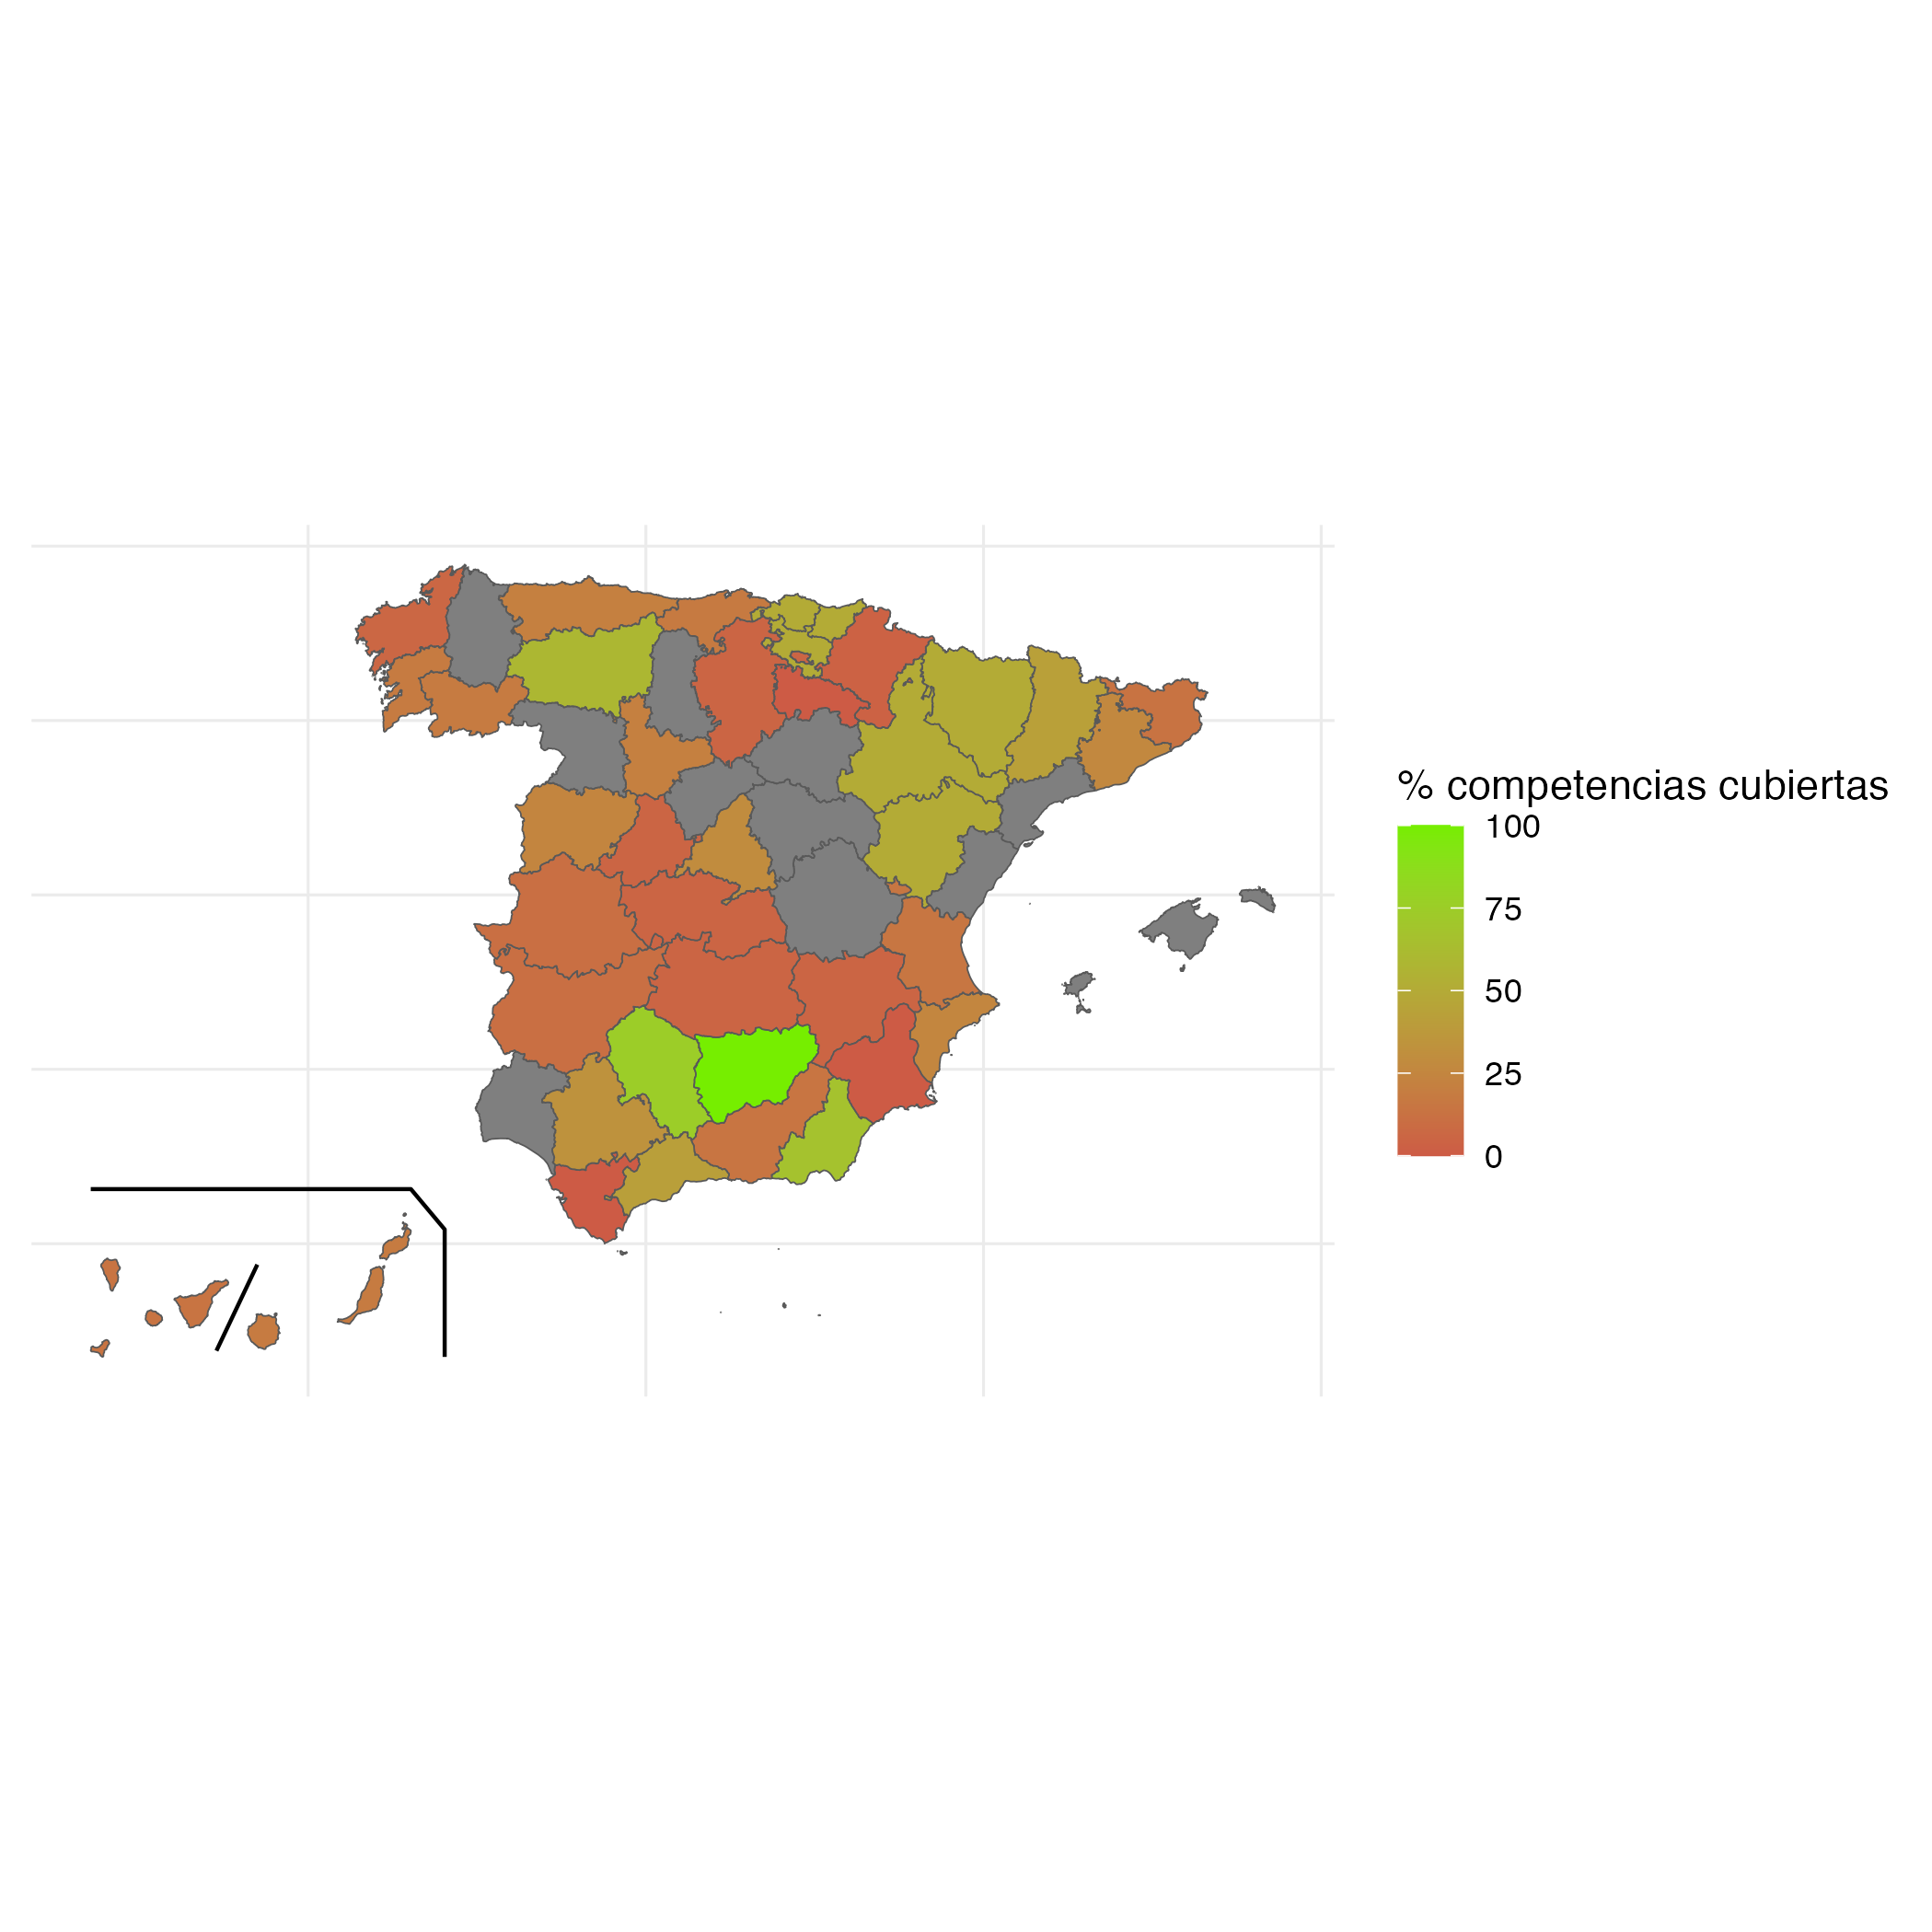
\includegraphics[scale=0.5, trim={0 5cm 5cm 5cm}, clip]{images/Mapa_prov.png}
        \captionof{figure}{Mapa de rúbricas basado en \cite{fernandez2023evaluacion}.}
        \label{fig:image}
    \end{minipage}
\end{table}

En caso de querer referenciar una página web, puedes hacerlo directamente en la bilbiografía con el resto de elementos. En caso de tener pocas referencias a páginas web puedes optar por incluirlas directamente como un pie de página o entre paréntesis. Ten en cuenta que dependiendo de la página web a la que hagas referencia puede ser necesario indicar el momento en que se ha accedido a esta información, especialmente si ésta se actualiza frecuentemente:

\begin{figure*}[!ht]
    \begin{minipage}{.45\textwidth}
        \begin{it}
        Para mas información puedes consultar la página web del Instituto Nacional de Estadística (https://ine.es/index.htm).
        \end{it}
    \end{minipage}
    \hfill
    \begin{minipage}{.45\textwidth}
        \begin{it}
        Para mas información puedes consultar la página web del Instituto Nacional de Estadística$^1$\\
        --\\
        $^1$ https://ine.es/index.htm. Accedido el 14 de febrero de 2024.
        \end{it}
    \end{minipage}
\end{figure*}

En caso de tener muchas referencias se recomienda tener un apartado de bibliografía exclusivo para los enlaces web y simplemente usar una referencia en el texto:

\begin{quote}
\begin{it}
    Para mas información puedes consultar la página web del Instituto Nacional de Estadística \cite{INE}.
\end{it}
\end{quote}

\begin{table}[!hbt]
    \centering
    \begin{minipage}{0.48\linewidth}
        \centering    
        \begin{tabular}{r|l}
            \toprule
            Referencia a & Información \\
            \midrule
            Libro & Autores/as \\
            & Título \\
            & Editorial \\
            & Año de publicación \\
            & {\it ISBN} \\
            & {\it Edición} \\
            \midrule
            Capítulo & Autores/as\\
            de Libro & Título del libro\\
            & Título del capítulo\\
            & Editorial\\
            & Año de publicación\\
            & {\it ISBN} \\
            & {\it Edición} \\
            \midrule
            Artículo & Autores/as\\
            científico & Título\\
            en revista & Nombre de la revista\\
            & Volumen \\
            & Año de publicación\\
            & {\it Número} \\  
            & {\it Páginas} \\
            & {\it DOI} \\
            \bottomrule
        \end{tabular}
    \end{minipage}%
    \hfill
    \begin{minipage}{0.48\linewidth}
        \centering
        \begin{tabular}{r|l}
            \toprule
            Referencia a & Información \\
            \midrule
            Artículo & Autores/as\\
            científico & Título\\
            en congreso & Nombre del congreso\\
            & Año de publicación\\
            & {\it Lugar} \\
            & {\it Fechas} \\
            & {\it Páginas} \\
            \midrule
            TFG & Autor/a\\
            TFM & Título \\
            Tesis doctoral & Universidad \\
            & Tipo \\
            & Año de publicación \\
            & {\it Tutor} \\
            \midrule
            Software & Nombre \\
            & Versión \\
            & {\it Enlace web} \\
            \midrule
            Página web & Título \\
            & Autores \\
            & Enlace web \\
            & Fecha de último acceso \\
            \bottomrule
        \end{tabular}
    \end{minipage}
    \caption{Información mínima y opcional (en itálica) para cada tipo de referencia a citar.}
    \label{tab:citar}
\end{table}

Si bien tienes estas tres opciones para referenciar contenido en línea, no debes usar más de una en tu memoria, elige la más conveniente y usa ese estilo para todas las referencias.

Si necesitas citar un software específico recuerda indicar la versión utilizada. Puedes adicionalmente agregar si quieres una referencia a la página web de la empresa o proyecto relacionado:

\begin{quote}
\begin{it}
    Para este trabajo se ha utilizado el lenguaje de programación Julia v1.10.0 (https://julialang.org/) \cite{bezanson2017julia}.
\end{it}
\end{quote}

En caso de reutilizar código fuente de otras personas indícalo tanto en el texto de la memoria, enlazando con la página web de donde has descargado esa información, como en tu propio código fuente mediante un comentario en la cabecera de la función o paquete donde se encuentre.

\begin{quote}
\begin{it}
    En este trabajo se ha reutilizado parte del código fuente del proyecto TSFEDL (\url{https://github.com/ari-dasci/S-TSFE-DL}), más detalles en el repositorio GitHub de este trabajo fin de grado (\url{https://github.com/mitfg/}).
\end{it}
\end{quote}

Para el resto de referencias, sean libros, artículos científicos u otros trabajos fin de carrera, la referencia bibliográfica deberá tener unos u otros componentes básicos dependiendo del tipo de referencia. En la Tabla \ref{tab:citar} puedes ver la información mínima y opcional (en itálica) para cada tipo de cita posible.
    
\begin{naranja}
Existen muchos formatos de citas, algunas usan números entre corchetes para referenciarlos, otros utilizan el nombre del primer autor y el año entre paréntesis, etc. Luego, dependiendo del formato se colocarán las referencias en la bibliografía en un cierto orden: orden alfabético, en el orden en que fueron citadas, etc. Estos formatos siguen distintas normativas o estilos. Las más conocidas son:

\begin{itemize}
    \item APA (American Psychological Association): En este formato, las referencias en el texto utilizan un sistema de citación por autor y fecha. Todas las citas que aparecen en el texto deberán luego ordenarse alfabéticamente. Este estilo se diseñó originalmente para trabajos en psicología, pero se han extendido a otros campos como la educación y las ciencias sociales debido a su claridad y facilidad de uso. Un ejemplo de este formato es:
    \begin{quote}
        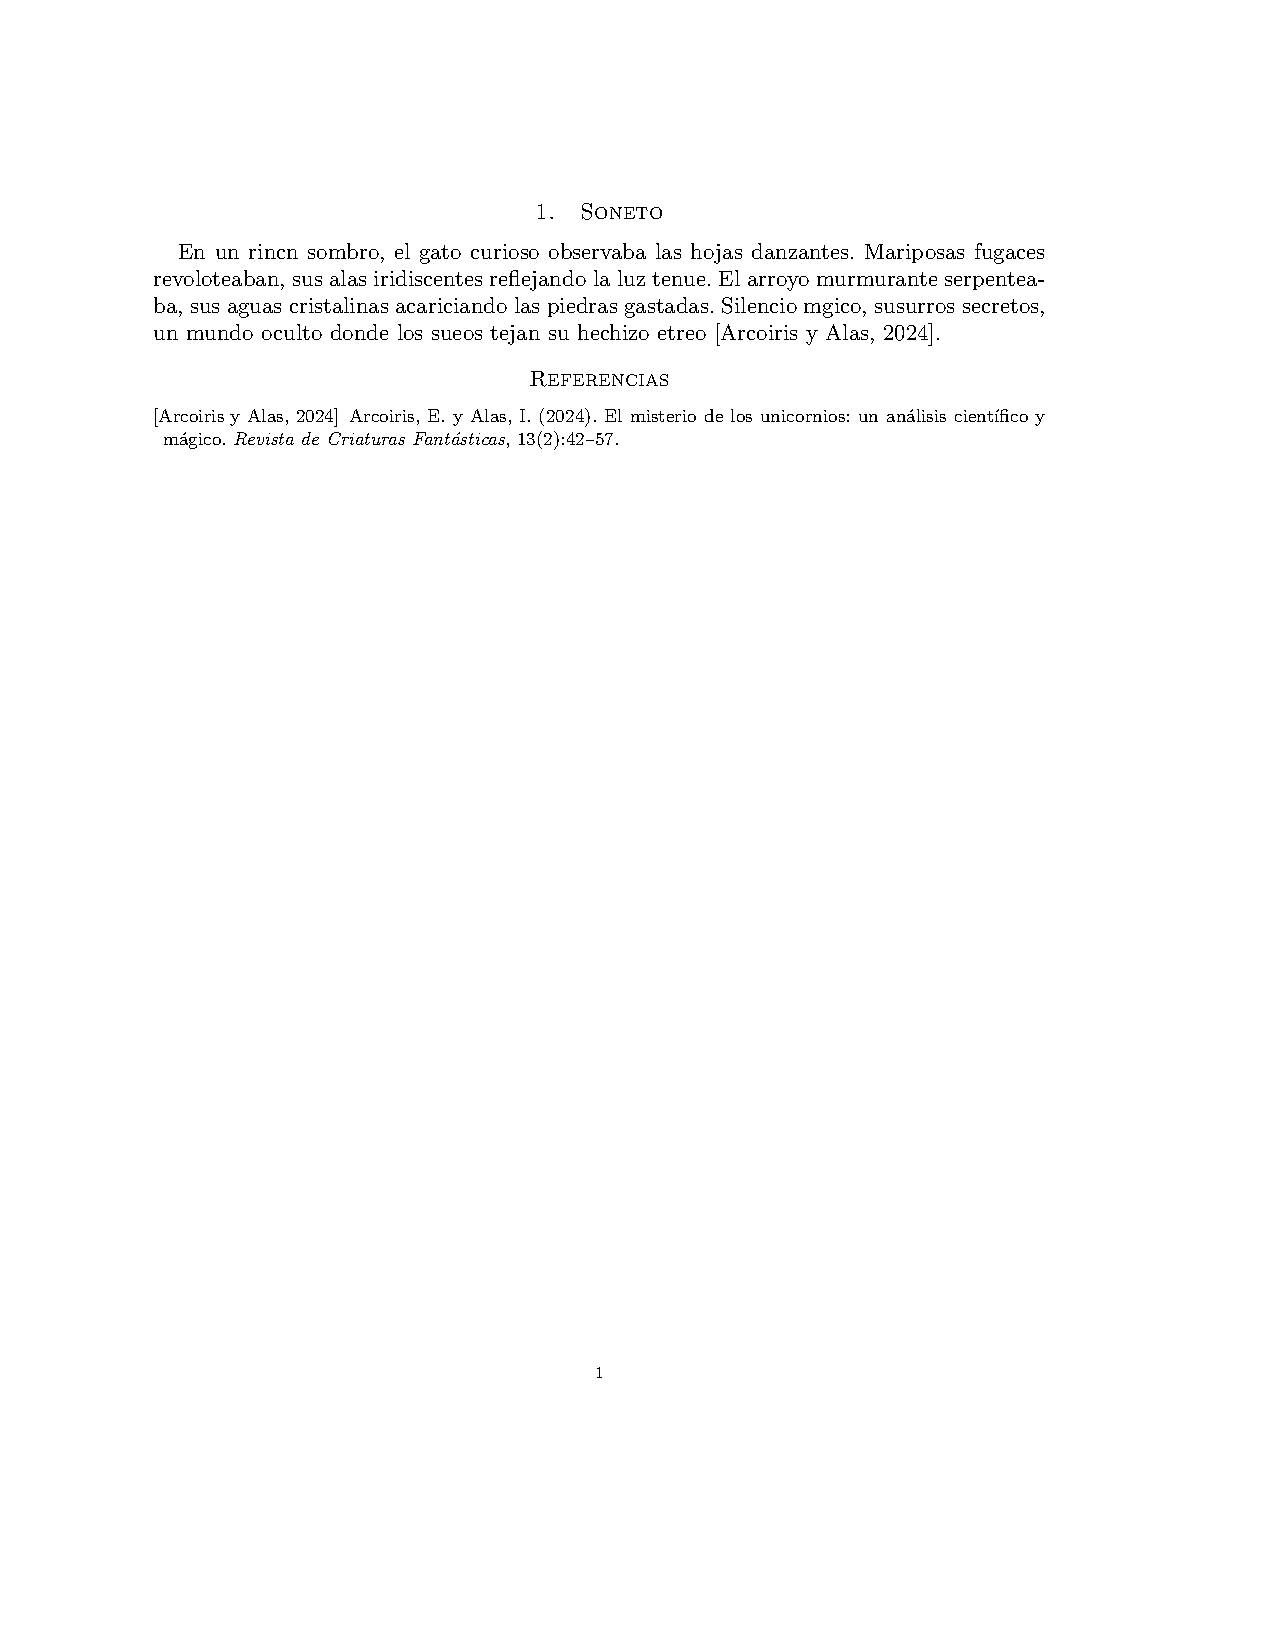
\includegraphics[scale=0.6, trim={2cm 20cm 3cm 3cm}, clip]{images/apa.pdf}
    \end{quote}
    \item MLA (Modern Language Association): En este formato, las citas dentro del texto no incluyen la fecha como en otros estilos, solo llevan el nombre del primer autor entre paréntesis. Es ampliamente utilizado en el ámbito de las humanidades, lengua y literatura. Un ejemplo de este formato es:
    \begin{quote}
        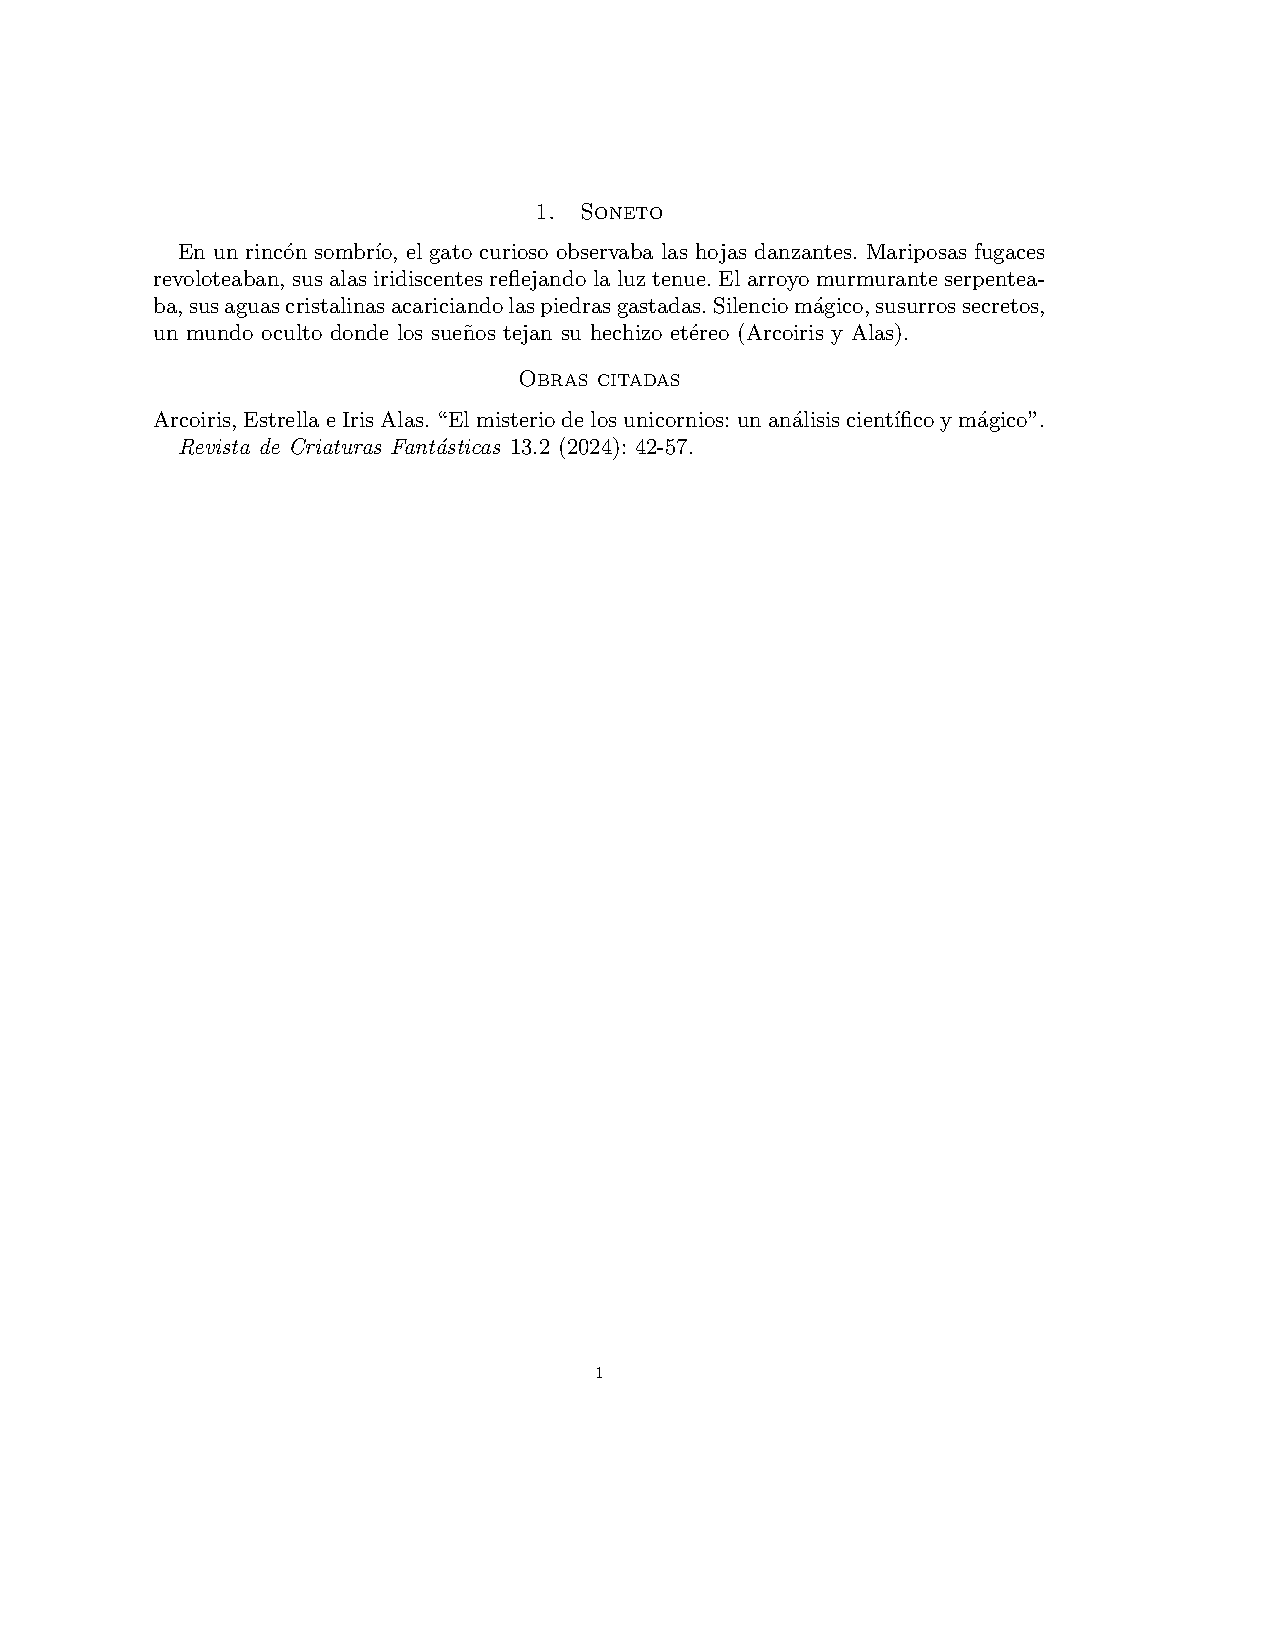
\includegraphics[scale=0.6, trim={2cm 20cm 3cm 3cm}, clip]{images/mla.pdf}
    \end{quote}
    \item Chicago: Este estilo tiene la posibilidad de formatear las citas de dos maneras diferentes: utilizando autor y fecha o con una nota al pie. Debe su nombre a la Universidad de Chicago donde fue creado y se emplea para citar en publicaciones científicas y académicas de distintos campos de humanidades, ciencias sociales y naturales. Un ejemplo de este formato es:
    \begin{quote}
        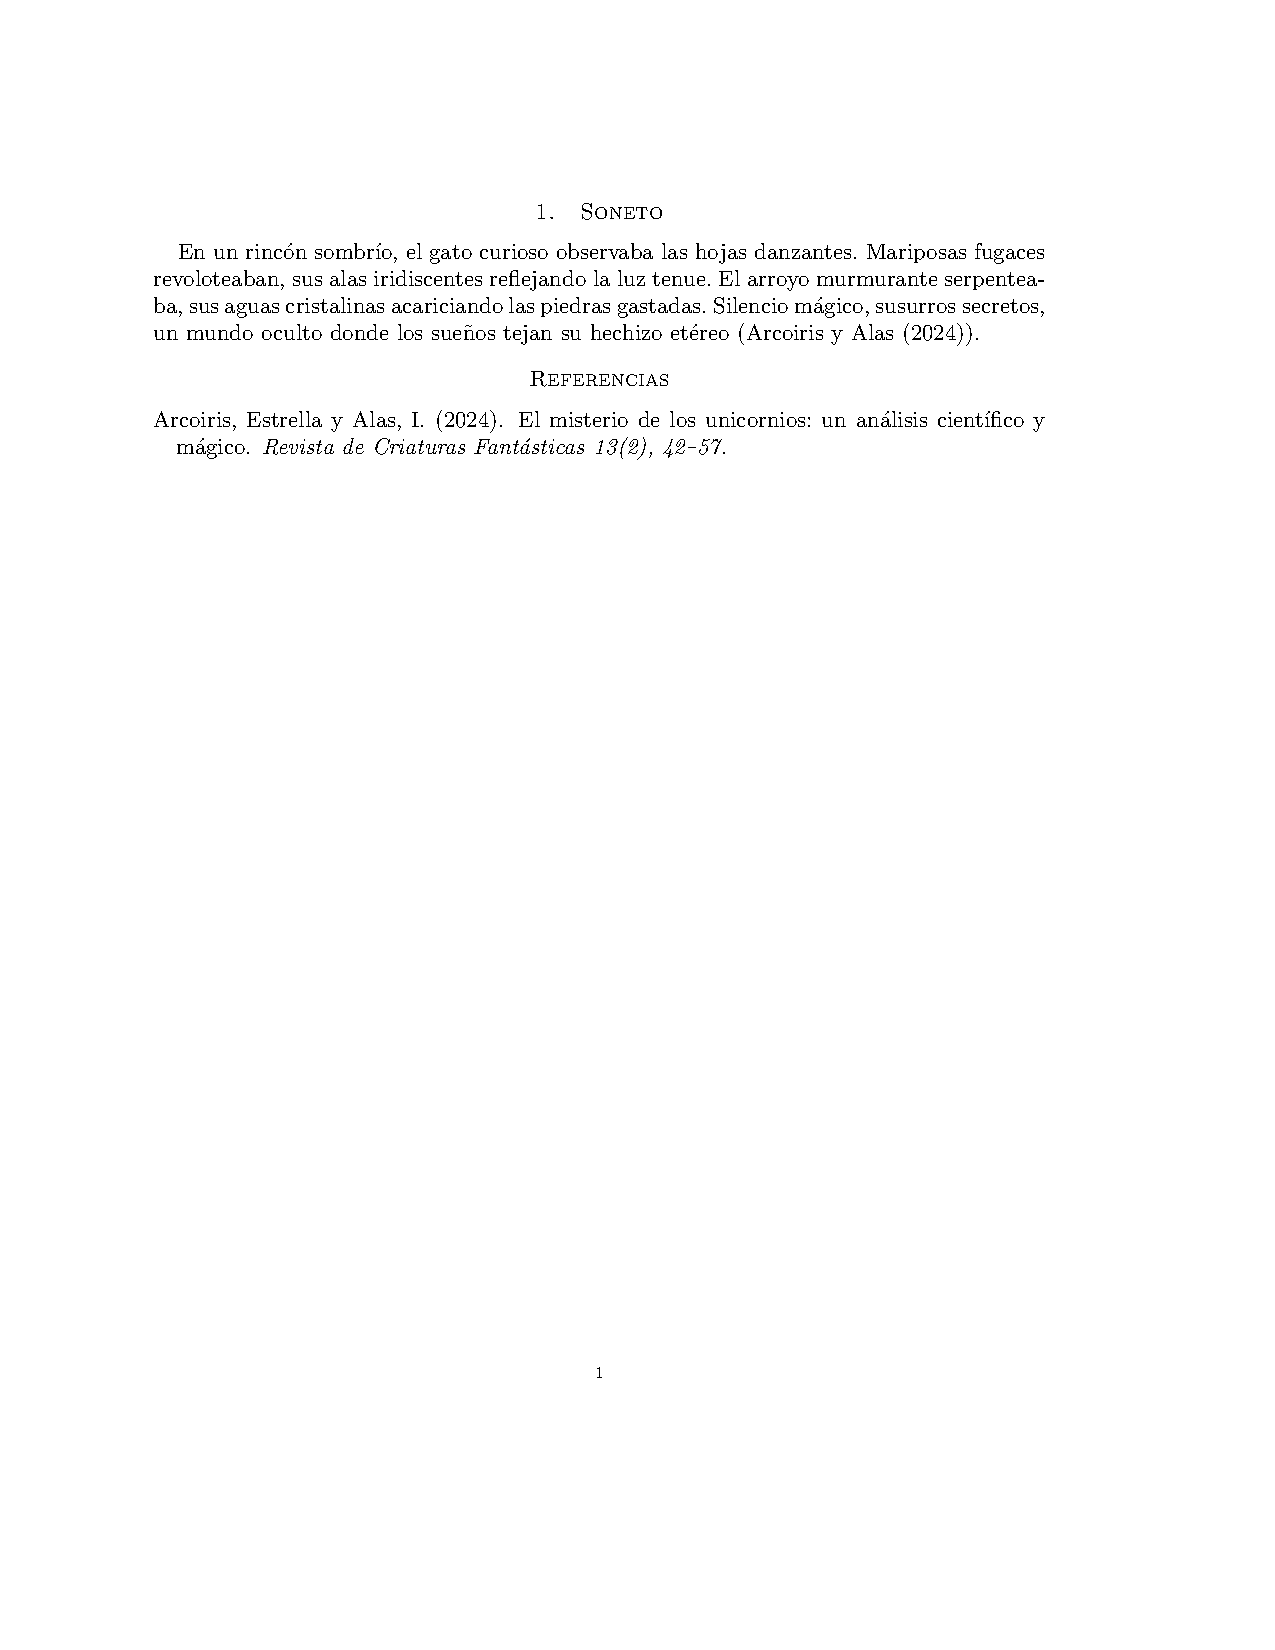
\includegraphics[scale=0.6, trim={2cm 20cm 3cm 3cm}, clip]{images/chicagoA.pdf}
    \end{quote}
    \item Harvard: Aunque este formato tiene su origen en la zoología y la biología en general, también es utilizado por los/las investigadores/as de distintas disciplinas como las ciencias sociales, la historia y las humanidades. Este sistema utiliza la información del autor-fecha para identificar una referencia bibliográfica. Un ejemplo de este formato es:
    \begin{quote}
        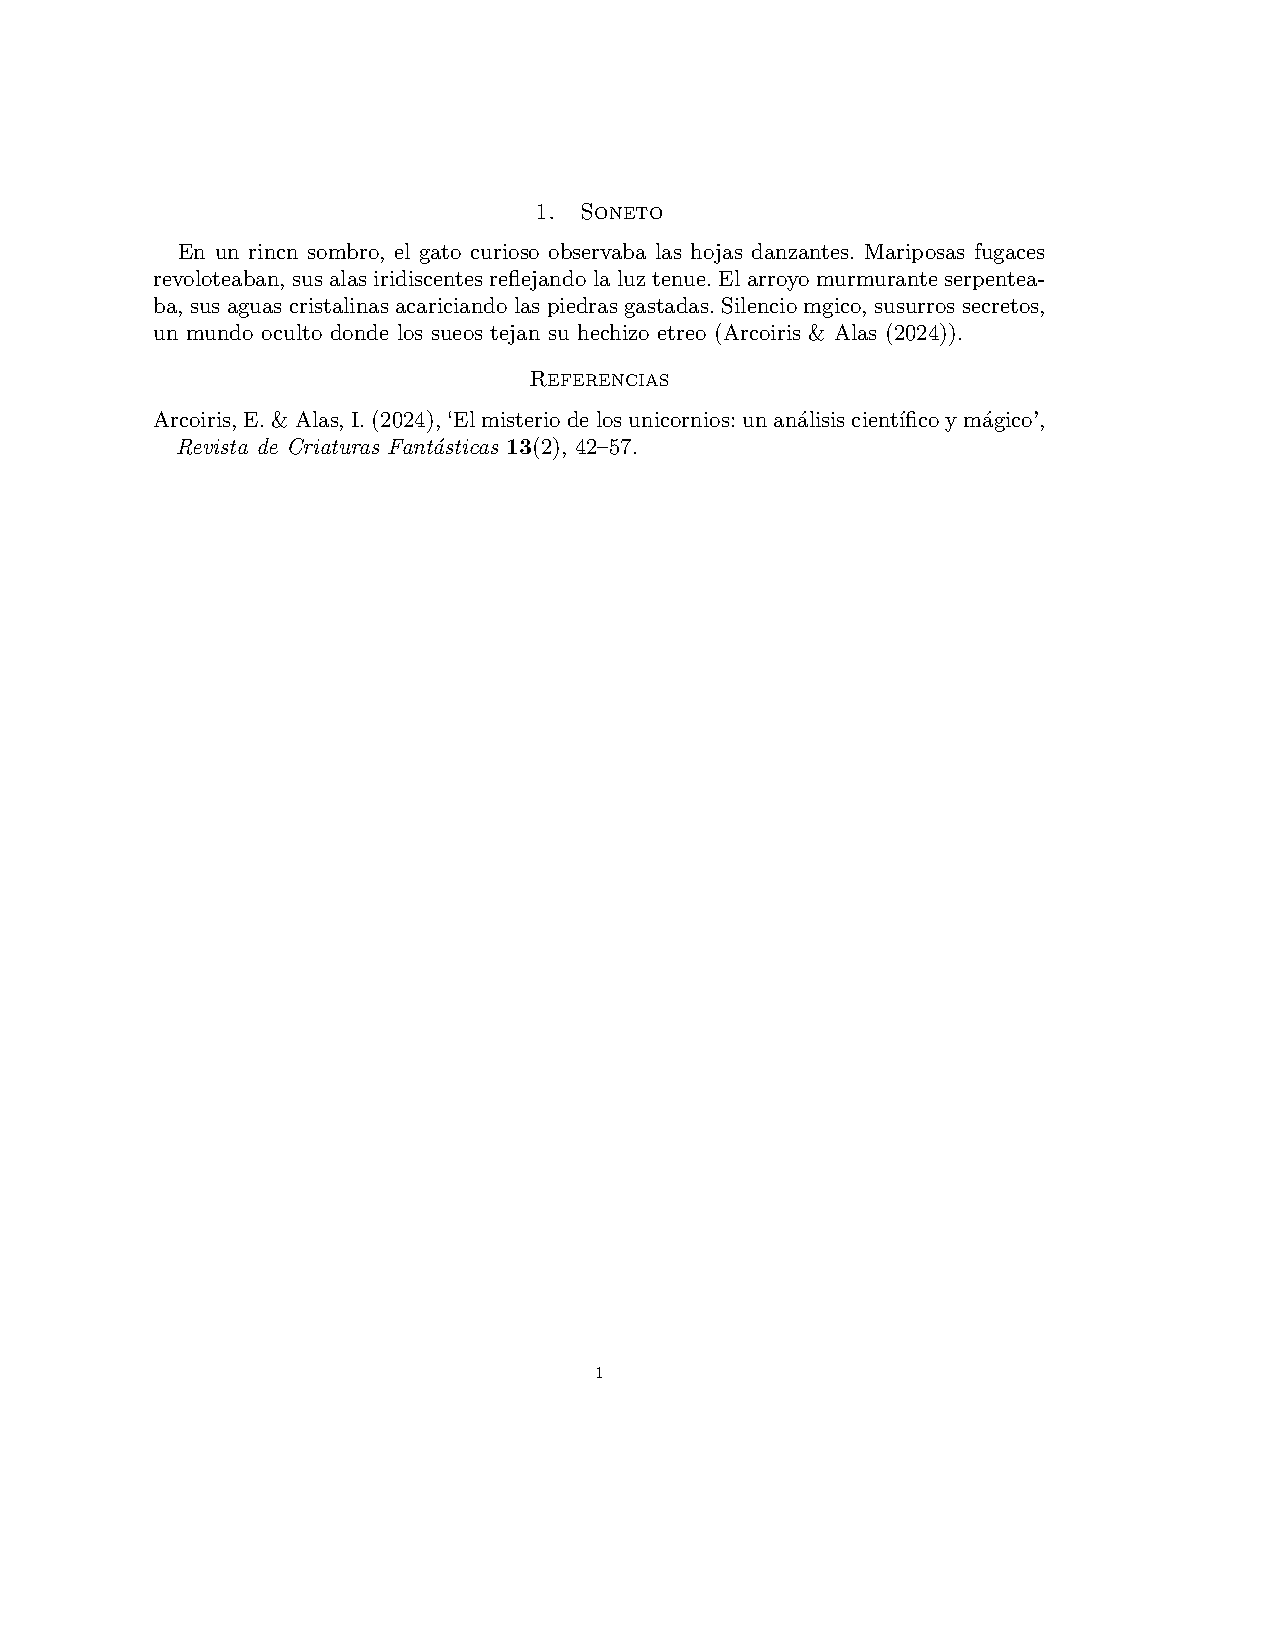
\includegraphics[scale=0.6, trim={2cm 20cm 3cm 3cm}, clip]{images/harvard.pdf}
    \end{quote}
    \item IEEE: En el estilo del Instituto de Ingenieros Eléctricos y Electrónicos (IEEE) las citas están numeradas entre corchetes. Toda la información bibliográfica se incluye exclusivamente en la lista de referencias al final del documento, junto al número de cita respectivo. Es el formato más utlizado en las ingenierías. Un ejemplo de este formato es:
    \begin{quote}
        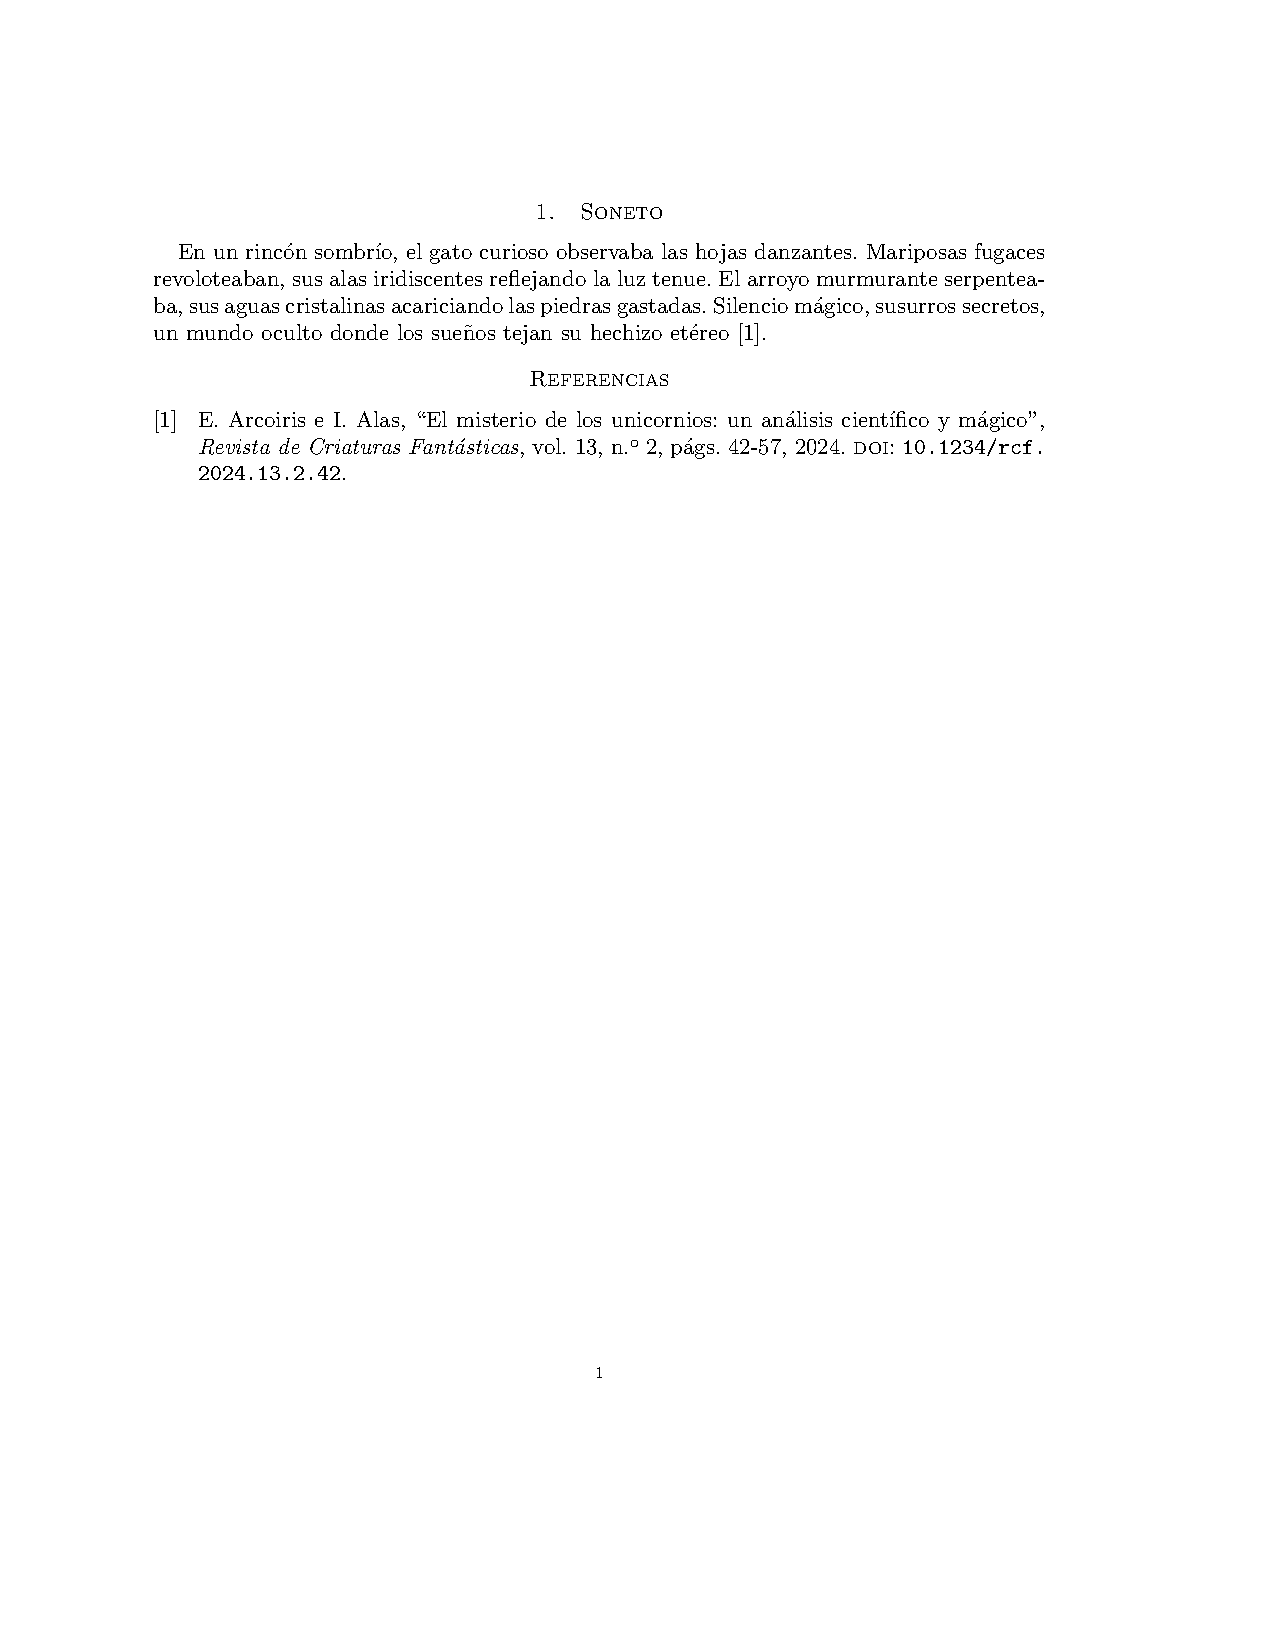
\includegraphics[scale=0.6, trim={2cm 19cm 3cm 3cm}, clip]{images/ieee.pdf}
    \end{quote}
\end{itemize}
\end{naranja}
Tienes libertad para elegir el estilo que más te guste, siempre y cuando utilices el mismo formato para toda la memoria. No puedes combinar distintos formatos en un solo documento.

\section{Herramientas de gestión de referencias y citas}

Organizar las citas y la bibliografía a mano no es nada recomendable. Imagina que cada vez que agregas una nueva cita tienes que ponerla en la bibliografía en la posición correcta y revisar que el formato sea el adecuado al estilo de citas que has elegido. Es por ello que existen muchas herramientas para poder tener las referencias controladas y accesibles. Dependiendo de que programa uses para escribir la memoria (e.g., Microsoft Word\texttrademark, \LaTeX\ u OpenOffice) tendrás disponibles unas u otras herramientas. La mayoría de los sistema de gestión de referencias y citas, sin embargo, suelen funcionar para cualquiera gracias a la posibilidad de importar y exportar las referencias en distintos formatos.

Los gestores de referencias y citas más populares son: EndNote (\url{https://endnote.com/es/}), Zotero (\url{https://www.zotero.org/}) y Mendeley (\url{https://www.mendeley.com/}). EndNote es una de las herramienta más completas y cómodas de usar, pero es una herramienta propietaria y es de pago. Mendeley es gratuita y te permite exportar conjuntos de bibliografías rápidamente. Zotero es la única de esta lista que es de código abierto. Existen muchas otras herramientas disponibles para descargar en Internet, con lo que te animo a explorar un poco más y elegir aquella que más cómoda te resulte. Verás la diferencia que hay entre utilizarla o tener que pasar horas poniendo las referencias y citas a mano.

En el caso de \LaTeX\ lo más apropiado es utilizar BibTeX. BibTeX es una herramienta y un formato de archivo para gestionar listas de referencias en documentos \LaTeX. Su función principal es generar automáticamente las citas y la lista de referencias en el formato seleccionado (e.g., APA, MLA, IEEE). También puedes utilizar herramientas independientes para la gestion de referencias y citas, como Mendeley, y combinarlas con \LaTeX\ y BibTeX.

\section{Consejos prácticos}

Como ya mencionamos, citar otras fuentes te permite respaldar tus argumentos. Es por ello que es imprescindible que utilices fuentes de información actualizadas, relevantes y confiables. Evita lo más posible citar la Wikipedia o Blogs de Internet no fiables. Intenta en su lugar cambiarlos por citas a libros o artículos científicos.

%No utilices generadores automáticos de texto, como ChatGPT, para buscar referencias. Muchos de ellos no están conectados a Internet, e incluso los que lo hacen pueden inventarse las referencias. Debes mantener el rigor científico en las citas que selecciones para tu memoria.

No incluyas bibliografía que nunca cites en el texto. Si bien el sistema de BibTeX controla esto, no todos los gestores lo hacen. Recuerda revisar tu memoria una vez finalizada para detectar estos problemas antes de entregarla.

Es fundamental citar las fuentes que has utilizado en tu trabajo. Si no lo haces, tu texto podría considerarse plagio y acarrear consecuencias graves.

Mantén un registro organizado de las referencias usadas desde el comienzo de tu trabajo y actualiza la bibliografía a medida que avanzas en tu proyecto. No lo dejes para el último momento ya que es posible que llegado a ese punto te hayas olvidado de las fuentes de donde hayas sacado la información y tengas que perder el tiempo volviéndolas a buscar.

Por último recordarte que uno de los aspectos a valorar en el baremo de los trabajos fin de grado y máster incluyen un apartado relacionado con la búsqueda y tratamiento de la información. En particular se tiene en cuenta la calidad, cantidad y variedad de las fuentes, pero también su adecuación y fiabilidad. 
